\documentclass[preview=true, border=10pt]{standalone}
%%%<
\usepackage{verbatim}
%%%>
\usepackage{tikz}
\usetikzlibrary{calc,positioning,shadows.blur,decorations.pathreplacing}
\usepackage{etoolbox}
\usepackage{siunitx}
\usepackage{nicefrac}

\definecolor{TrueData}{HTML}{d95f02}
\definecolor{Simulation}{HTML}{1b9e77}

\newcommand{\LHCbSoftTikzSize}{1.2}

\newcommand\Softwarepackage[2][TrueData]{%
  \begin{tikzpicture}[x=\LHCbSoftTikzSize cm, y=\LHCbSoftTikzSize cm]
    \path[fill=#1] (0.1*\LHCbSoftTikzSize,0) -- (0.9,0)
        arc (90:0:0.1*\LHCbSoftTikzSize cm) -- (1.0,-0.9) arc (0:-90:0.1*\LHCbSoftTikzSize cm) -- (0.1,-1.0)
        arc (-90:-180:0.1*\LHCbSoftTikzSize cm) -- (0,-0.1) arc(180:90:0.1*\LHCbSoftTikzSize cm) -- cycle;
    \ifstrempty{#2}{}{\node at(0.5,-0.5)  [nosep,anchor=center,scale=0.588*\LHCbSoftTikzSize,color=white] {#2};}
  \end{tikzpicture}
}

\newcommand\DataFormat[2][TrueData]{%
  \begin{tikzpicture}[x=\LHCbSoftTikzSize cm, y=\LHCbSoftTikzSize cm]
    \path[fill=#1] (0.5,0) arc (90:0:0.5*\LHCbSoftTikzSize cm) -- (1.0,-0.5) arc (0:-90:0.5*\LHCbSoftTikzSize cm)
                  -- (0.5, -1.0) arc (-90:-180:0.5*\LHCbSoftTikzSize cm) -- (0,-0.5) arc(180:90:0.5*\LHCbSoftTikzSize cm) -- cycle;
    \ifstrempty{#2}{}{\node at(0.5,-0.5)  [nosep,anchor=center,scale=0.588*\LHCbSoftTikzSize,color=white] {#2};}
  \end{tikzpicture}
}

\newcommand\DetectorBox[1]{%
  \begin{tikzpicture}[x=\LHCbSoftTikzSize cm, y=\LHCbSoftTikzSize cm]
    \path[fill=black] (0.5,0) -- (1.0,-0.5) -- (0.5, -1.0) -- (0,-0.5) -- cycle;
    \node at(0.5,-0.5)  [nosep,anchor=center,scale=0.706*\LHCbSoftTikzSize,color=white] {#1};
  \end{tikzpicture}
}

\newcommand\SimulationBox[1]{%
  \begin{tikzpicture}[x=\LHCbSoftTikzSize cm, y=\LHCbSoftTikzSize cm]
    \path[fill=black] (0.0,0) -- (1.5,0.0) -- (1.5, -0.7) -- (0.0, -0.7) -- cycle;
    \node at(0.75,-0.35)  [nosep,anchor=center,scale=0.706*\LHCbSoftTikzSize,color=white] {#1};
  \end{tikzpicture}
}

\begin{document}
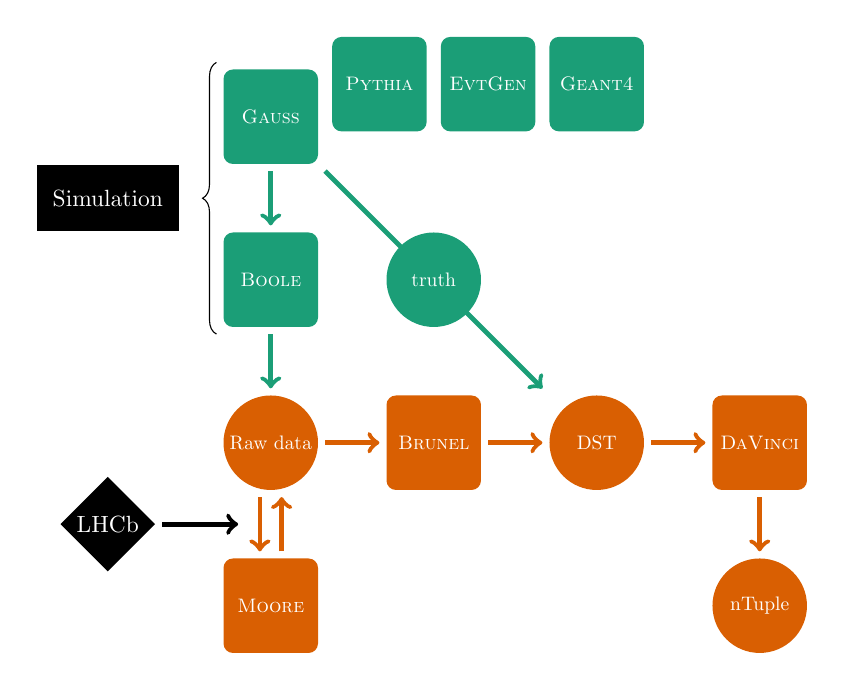
\begin{tikzpicture}[x=1.15*\LHCbSoftTikzSize cm, y=1.15*\LHCbSoftTikzSize cm,
                    round/.style = { rounded corners=2mm },
                    brace/.style = { decorate, decoration={brace, amplitude=5pt} },
                    mbrace/.style = { decorate, decoration={brace, amplitude=5pt, mirror} },
                    label/.style = { black, midway, scale=0.5, align=center },
                    toplabel/.style = { label, above=.5em, anchor=south },
                    leftlabel/.style = { label,rotate=-90,left=.5em,anchor=north },
                    bottomlabel/.style = { label, below=.5em, anchor=north },
                    force/.style = { rotate=-90,scale=0.8 },
                    legend/.style = { right,scale=0.4 },
                    nosep/.style = { inner sep=0pt },
                    generation/.style = { anchor=base }]

  \node at(0, 0)   {\DataFormat{Raw data}};
  \node at(0,-1.5)   {\Softwarepackage{\textsc{Moore}}};
  \node at(1.5, 0)   {\Softwarepackage{\textsc{Brunel}}};
  \node at(3, 0)   {\DataFormat{DST}};
  \node at(4.5, 0)   {\Softwarepackage{\textsc{DaVinci}}};
  \node at(4.5,-1.5)   {\DataFormat{nTuple}};
  \node at(0, 1.5)   {\Softwarepackage[Simulation]{\textsc{Boole}}};
  \node at(0, 3)   {\Softwarepackage[Simulation]{\textsc{Gauss}}};
  \node at(1, 3.3)   {\Softwarepackage[Simulation]{\textsc{Pythia}}};
  \node at(2, 3.3)   {\Softwarepackage[Simulation]{\textsc{EvtGen}}};
  \node at(3, 3.3)   {\Softwarepackage[Simulation]{\textsc{Geant4}}};

  \node at(-1.5,-0.75)   {\DetectorBox{LHCb}};
  \node at(-1.5, 2.25)   {\SimulationBox{Simulation}};

  \draw [->, color=TrueData, line width=\LHCbSoftTikzSize * 0.5mm] (0.5, 0) -- (1.0, 0);
  \draw [->, color=TrueData, line width=\LHCbSoftTikzSize * 0.5mm] (2.0, 0) -- (2.5, 0);
  \draw [->, color=TrueData, line width=\LHCbSoftTikzSize * 0.5mm] (3.5, 0) -- (4.0, 0);
  \draw [->, color=TrueData, line width=\LHCbSoftTikzSize * 0.5mm] (4.5, -0.5) -- (4.5, -1.0);
  \draw [->, color=TrueData, line width=\LHCbSoftTikzSize * 0.5mm] (-0.1, -0.5) -- (-0.1, -1.0);
  \draw [->, color=TrueData, line width=\LHCbSoftTikzSize * 0.5mm] (0.1, -1.0) -- (0.1, -0.5);
  \draw [->, color=black, line width=\LHCbSoftTikzSize * 0.5mm] (-1.0, -0.75) -- (-0.3, -0.75);

  \draw [->, color=Simulation, line width=\LHCbSoftTikzSize * 0.5mm] (0, 2.5) -- (0, 2.0);
  \draw [->, color=Simulation, line width=\LHCbSoftTikzSize * 0.5mm] (0, 1.0) -- (0, 0.5);

  \draw [->, color=Simulation, line width=\LHCbSoftTikzSize * 0.5mm] (0.5, 2.5) -- (2.5, 0.5);
  \node at(1.5,1.5)   {\DataFormat[Simulation]{truth}};

  \draw [brace] (-0.5,1) -- (-0.5,3.5) node[leftlabel]{};
\end{tikzpicture}
\end{document}
